%%%%%%%%%%%%%%%%%%%%%%%%%%%%%%%%%%%%%%%%%%%%%%%%%%%%%%%%%%%%%%%%%%%%%%%%%%%%%%%%
%2345678901234567890123456789012345678901234567890123456789012345678901234567890
%        1         2         3         4         5         6         7         8

\documentclass[letterpaper, 10 pt, conference]{ieeeconf}  % Comment this line out if you need a4paper

%\documentclass[a4paper, 10pt, conference]{ieeeconf}      % Use this line for a4 paper

\IEEEoverridecommandlockouts                              % This command is only needed if 
                                                          % you want to use the \thanks command

\overrideIEEEmargins                                      % Needed to meet printer requirements.

%In case you encounter the following error:
%Error 1010 The PDF file may be corrupt (unable to open PDF file) OR
%Error 1000 An error occurred while parsing a contents stream. Unable to analyze the PDF file.
%This is a known problem with pdfLaTeX conversion filter. The file cannot be opened with acrobat reader
%Please use one of the alternatives below to circumvent this error by uncommenting one or the other
%\pdfobjcompresslevel=0
%\pdfminorversion=4

% See the \addtolength command later in the file to balance the column lengths
% on the last page of the document

% The following packages can be found on http:\\www.ctan.org
\usepackage{caption}
\captionsetup[table]{position=bottom}
\usepackage{listings}
\lstset{language=C}
\usepackage{graphicx}
\usepackage[backend=bibtex]{biblatex}
\addbibresource{literature.bib}

\title{\LARGE \bf
Report on ORB-SLAM: A Versatile and Accurate SLAM System
}


\author{Yuxuan Xue$^{1}$% <-this % stops a space
\thanks{$^{1}$Yuxuan Xue is with Faculty of Informatics and Mechanical Engineering,
        Technical University of Munich, 85748 Garching bei Munich, Germany
        {\tt\small yuxuan.xue@tum.de}}%
}

\begin{document}



\maketitle
\thispagestyle{empty}
\pagestyle{empty}


%%%%%%%%%%%%%%%%%%%%%%%%%%%%%%%%%%%%%%%%%%%%%%%%%%%%%%%%%%%%%%%%%%%%%%%%%%%%%%%%
\begin{abstract}

This paper is a report on ORB-SLAM, a topic in seminar sensors in robots. ORB-SLAM is a feature-based monocular simultaneous localization and mapping (SLAM) system that operates well-performed in real-time and in environments with different illumination or scaling conditions. This paper introduces how ORB-SLAM works from the algorithm level, the primary procedure, the comparison to other popular SLAM methods, and a lesson learned from the preparation of the presentation and the function implementation.


\end{abstract}


%%%%%%%%%%%%%%%%%%%%%%%%%%%%%%%%%%%%%%%%%%%%%%%%%%%%%%%%%%%%%%%%%%%%%%%%%%%%%%%%
\section{Introduction}
\label{section_introduction}

ORB-SLAM \cite{ORBSLAM} is a state-of-the-art visual SLAM method. As shown in figure \ref{main_structure}, the visual SLAM system consists of five modules. The camera captures images. The visual odometry (frontend) estimates camera motion based on images. The loop closure detector uses images to address the drifting problem of position estimation. The optimization step (backend) uses the information from visual odometry and loop closure detector to estimate uncertainty and eliminate accumulating drift. In the end, a map of the environment is generated according to the information from the backend.
%
\begin{figure}[!htbp]%
\centering
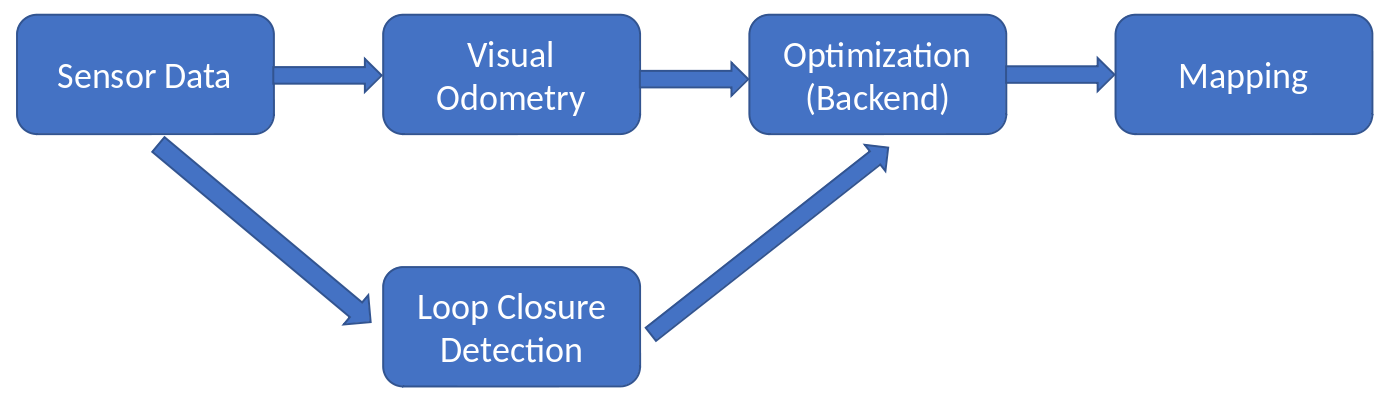
\includegraphics[scale=0.175]{./images/Main_structure}
\caption{A general structure of visual SLAM system consists of sensors, frontend, backend, loop closing, and mapping.}
\label{main_structure}
\end{figure}
%
\\

In comparison to previous SLAM methods, the ORB SLAM has the following main contributions.
\begin{itemize}


\item Features:  ORB features allow real-time performance without GPU and provide good invariance to changes in viewpoint and illumination. Use of the same features for all tasks makes SLAM system more efficient, simple and reliable. 
\item Covisibility Graph: Tracking and Mapping are only focused on a local covisible area. The use of covisibility graph ensures the SLAM system's real-time operation in a large environment, independent of global map size.
\item Essential Graph: A spanning tree maintained by the system, loop closure links, and strong edges from the covisibility graph. Thanks to the essential graph, the SLAM system has a real-time loop closing operation.
\item Camera relocalization: Thanks to significant invariance to viewpoint and illumination, the System can provide real-time recovery from tracking  failure and enhancing map reuse.
\item Map Initialization: A new approach to select a model for the planar and nonplanar case builds an automatic and robust initialization procedure. 
\item Map point and Keyframe selection: A reliable approach to select keyframe and map point improves tracking robustness, and ignore redundant keyframes.

\end{itemize}

\section{Technique}
\subsection{Parralel Tracking and Mapping}
Bundle adjustment (BA) is a well-known nonlinear optimization algorithm aiming at the minimization of reprojection error to provide accurate estimates of camera localization and points geometry reconstruction \cite{1},\cite{2}. However, due to the high cost of computation, the BA approach was considered unaffordable for real-time applications such as visual SLAM for a long time.

The first groundbreaking real-time SLAM using BA is parallel tracking and mapping (PTAM) \cite{PTAM} by Klein and Murray in 2007. This algorithm provides effective and straightforward methods for feature matching, point triangulation, and tracking failure.  However, it is limited to small-scale operation because it has no loop closing part and low invariance to the viewpoint of relocalization. ORB-SLAM is built on the main ideas of PTAM, and have a significant improvement on the Weakness.

\subsection{Place Recognition}
According to the survey by Williams \cite{13}, the image-to-image matching scales generally better than map-to-map or image-to-map methods. A bag of words technique DBoW2 \cite{14} is used for the first time bags of binary words obtained from BRIEF descriptors to reduce the time needed for feature extraction. 

\subsection{Keyframes and its selection}
Keyframe is an essential definition of ORB-SLAM. Many important procedures, such as triangulation of map points in local mapping and loop detection in loop closing, are based only on Keyframes. Generally, the less the Keyframes, the less the drift accumulated. However, if keyframes are too sparse, it has a high possibility of lost tracking. A reliable criterion to select keyframe is introduced in section \ref{section3}.

\subsection{Covisibility and Essential Graph}
Globally, a SLAM system can capture many keyframes. A proper way is to store these keyframes into a covisibility graph \cite{7}. Like its name, the covisibility graph build edge between two keyframes, when they have many covisible map points. Each edge has weight, which means how many covisible points the two keyframes have.

The essential graph is global. It simplifies the covisibility graph by subtracting edges with weights less than 100. By use of an essential graph, the loop closing can process more efficiently \cite{6}. The way to construct a covisibility graph and an essential graph is shown intuitively in figure \ref{covisibility_essential_graph}.
%
\begin{figure}[!htbp]%
\centering
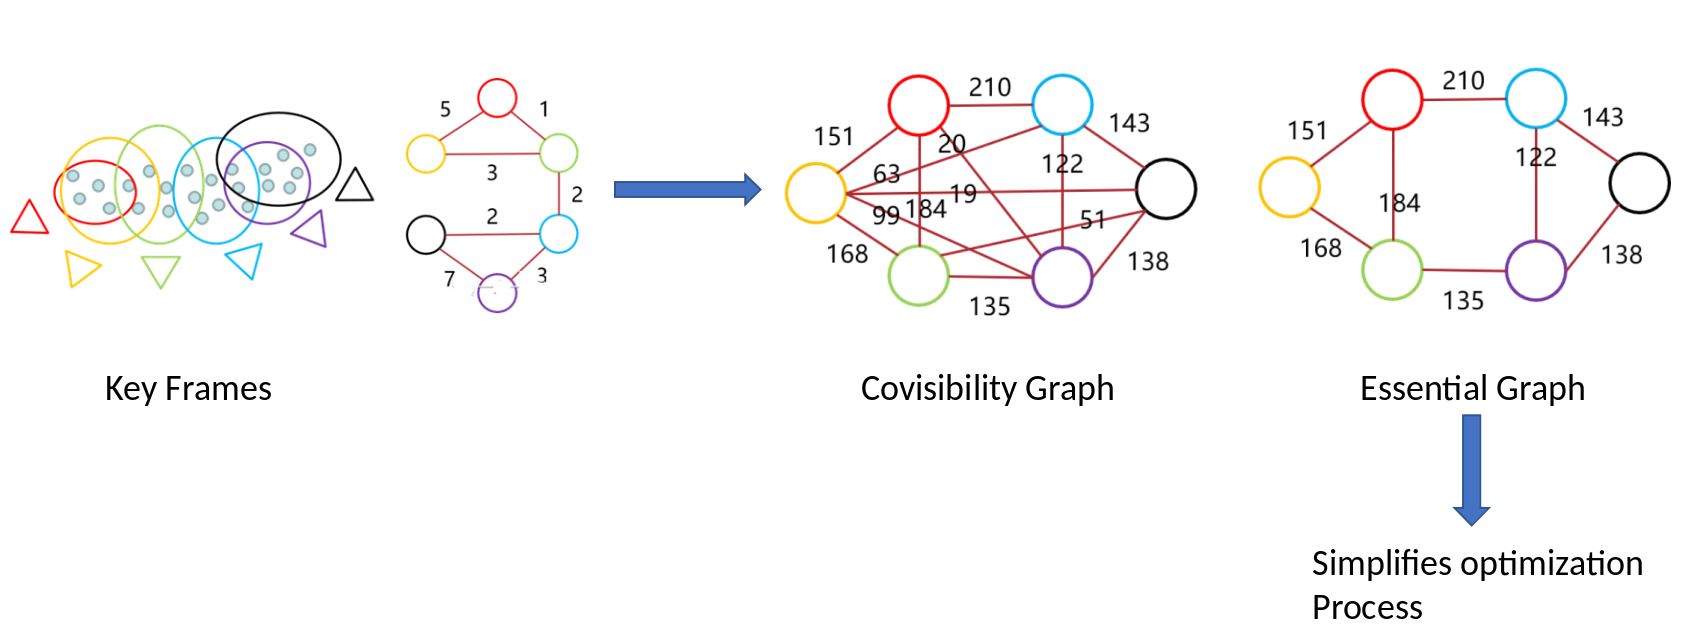
\includegraphics[scale=0.148]{./images/covisibility_essential_graph}
\caption{The mechanism of how to construct a covisibility graph from keyframes and how to construct an essential graph from the covisibility graph.}
\label{covisibility_essential_graph}
\end{figure}
%

\subsection{Feature Choice}
ORB feature is one of ORB-SLAM's main contributions. As shown in table \ref{feature_extraction_time} \cite{ORBextract}, Oriented FAST and Rotated BRIEF (ORB) has a tremendous advantage in computation efficiency over commonly used feature detector SIFT and SURF. The performance also meets the requirement of a real-time SLAM system.
%
\begin{table}[h!]
\caption{Feature extraction time of a single frame.}
\label{feature_extraction_time}
\centering
\begin{tabular}{ c c c c } 
 \hline
 \hline
 Detector & ORB & SIFT & SURF \\ 
 \hline
 Time per frame (ms)& 15.3 & 217.3 & 5228.7\\ 
 \hline
 \hline
\end{tabular}
\end{table}
%

Features from Accelerated Segment Test (FAST) detector has sufficient computation efficiency. However, FAST is not invariant to rotation and scaling. Figure \ref{oriented_fast} shows the procedure from normal FAST to a scale-invariant oriented FAST. 
%
\begin{figure}[!htbp]%
\centering
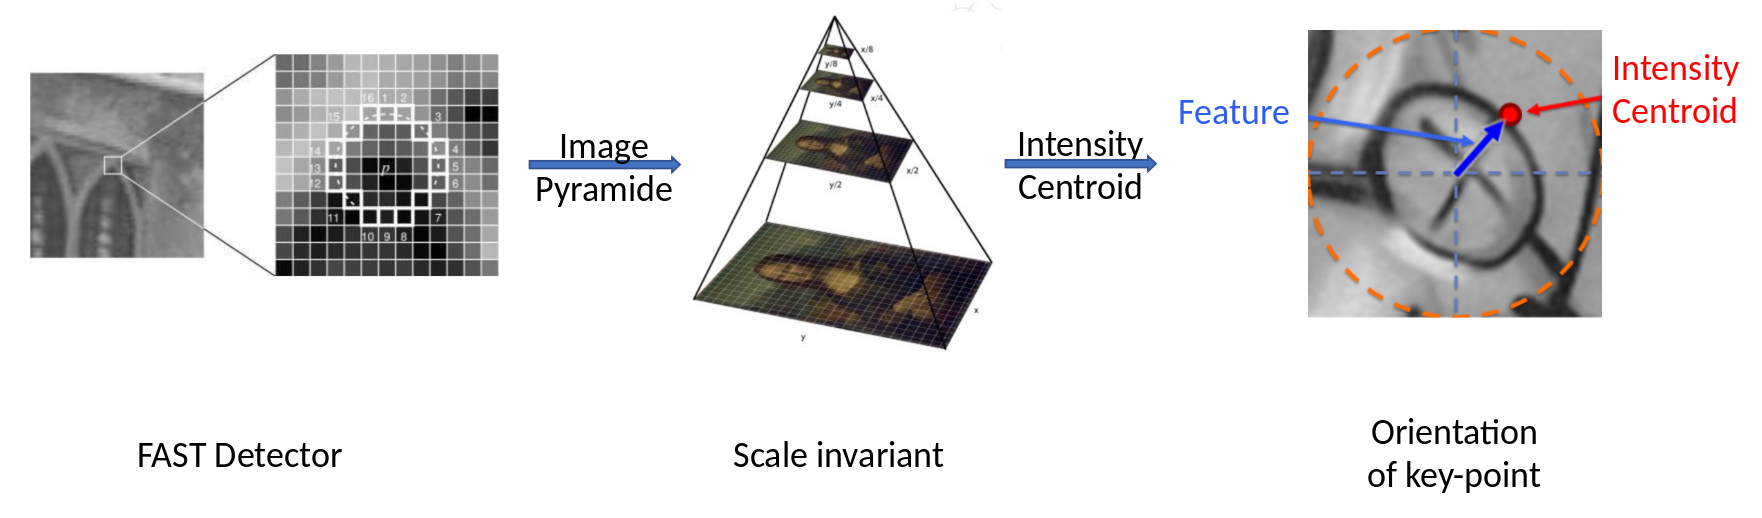
\includegraphics[scale=0.14]{./images/Oriented_FAST}
\caption{The procedure for building Oriented FAST. The Image pyramid makes FAST scale-invariant. Intensity centroid around feature point computes orientation and makes FAST rotation-invariant.}
\label{oriented_fast}
\end{figure}
%

Binary Robust Independent Elementary Features (BRIEF) is a feature descriptor, which describes the key-point with binary vector. Associated with the orientation from feature detector, BRIEF can describe key-point with orientation, which makes BRIEF to Oriented BRIEF. Figure\ref{point_correspondence} shows the matching result of 2 images using ORB.

%
\begin{figure}[!htbp]%
\centering
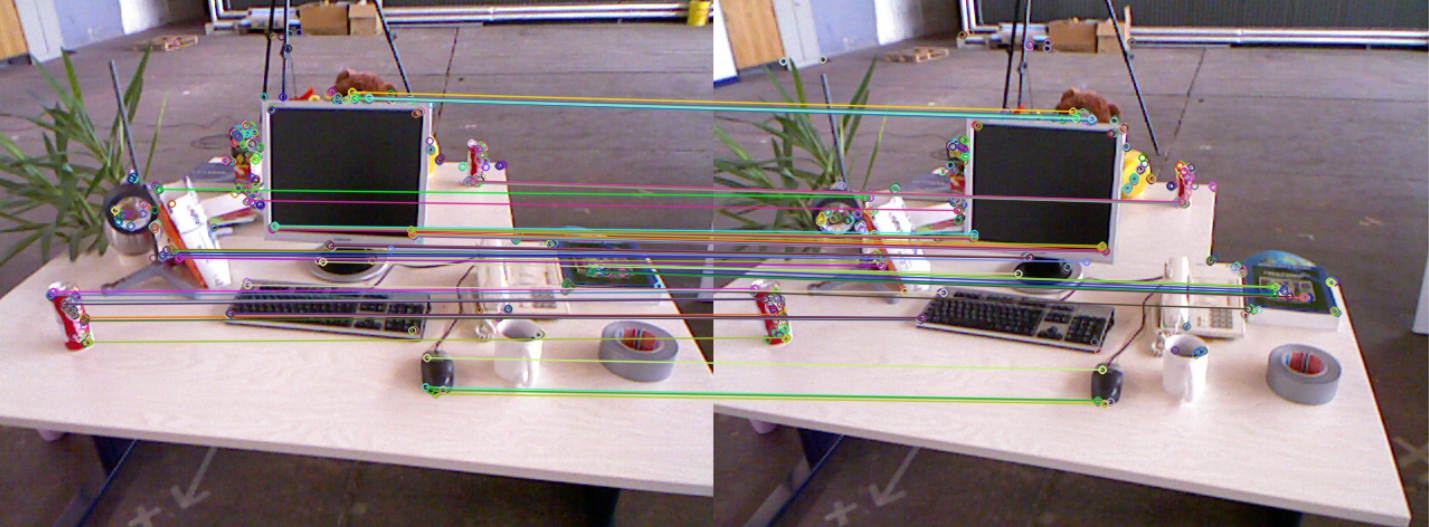
\includegraphics[scale=0.17]{./images/Point_correspondence}
\caption{Feature point matching using ORB. \cite{ORBextract}}
\label{point_correspondence}
\end{figure}
%

In general, ORB is extremely fast to compute and match. It is feasible to match points with a large baseline because it has good invariance to viewpoint. Due to these advantages, ORB is a perfect detector and descriptor in a real-time SLAM system. 

\section{System Overview}
\label{section3}
The ORB-SLAM system, see an overview in Figure \ref{system_overview}, contains three threads that run in parallel: tracking, local mapping, and loop closing.

\begin{figure}[!htbp]%
\centering
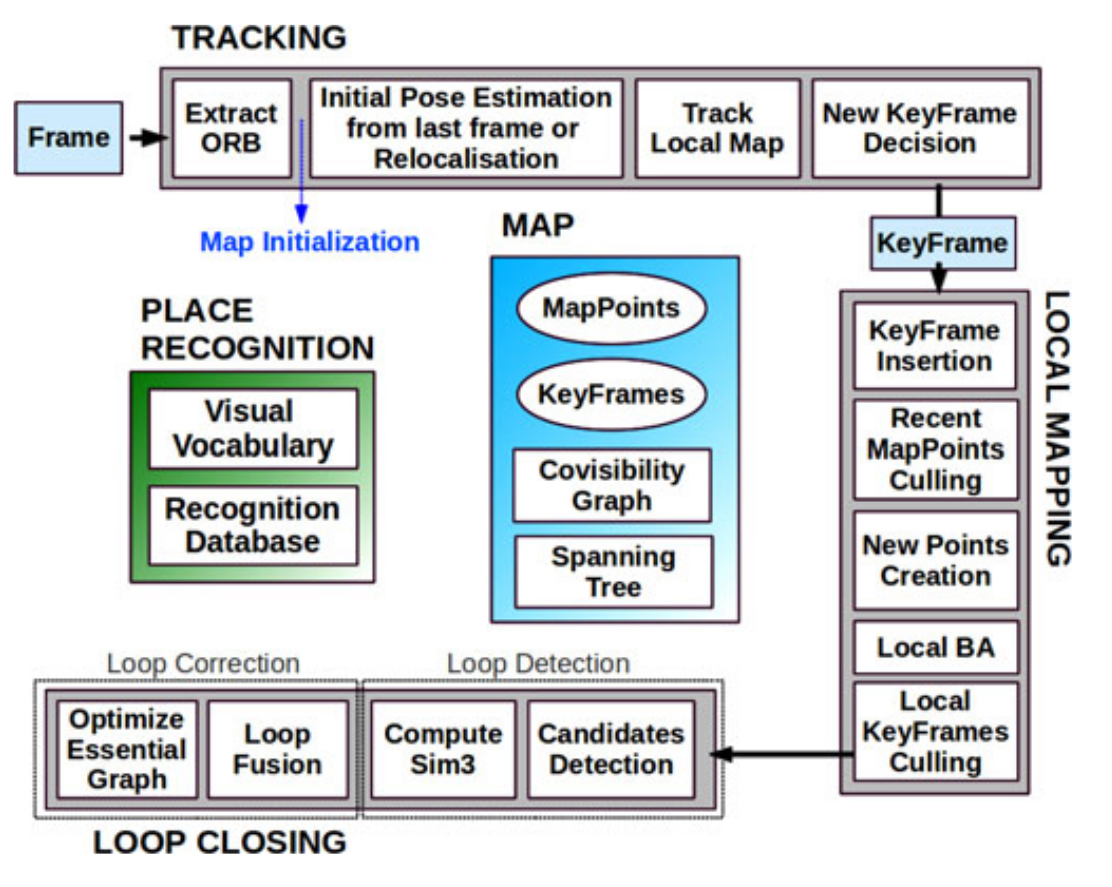
\includegraphics[scale=0.22]{./images/System_overview}
\caption{ORB-SLAM system overview, showing all the steps performed by the
tracking, local mapping, and loop closing threads. The main components of the
place recognition module and the map are also shown. \cite{ORBSLAM}}
\label{system_overview}
\end{figure}

In the tracking step, the SLAM system extracts ORB features and estimates the initial pose of the camera. In addition, once tracking is lost,  the place recognition module is used to perform a global reconstruction. In this step, the system also has to decide whether the current frame is a keyframe. 

Local mapping processes the information of keyframes. It performs a local BA to have an optimal reconstruction of the surrounding of the camera locally. The unmatched ORB features are searched in the covisibility graph to triangulate new map points, which is especially meaningful in the reconstruction step.

The loop closing searches for loops with every new keyframe. Once a loop is detected, the system computes a similarity transformation to calculate the drift accumulated in the loop. Duplicated map points are fused according to the accumulated drift.


\subsection{Tracking}
Tracking thread performs with every frame from the camera. It consists of several steps.
\subsubsection{Automatic Map Initialization}
\label{map_init}
As known to all, the BA method needs proper initialization. The goal of the map initialization is to compute relative pose between two frames and triangulate an initial set of map points.

There are two models in general: Homography $\textbf{H}_{cr}$ for planar scene and fundamental matrix $\textbf{F}_{cr}$ for nonplanar scene \cite{2}. The system computes the score for each model M simultaneously with equation
%
\begin{equation}
S_M = \sum_i(\rho_M(d_{cr}^2(x_c^i,x_r^i,M)))+\rho_M(d_{rc}^2(x_c^i, x_r^i, M))
\end{equation}
%
Then a robust heuristc is found to compute
%
\begin{equation}
R_H = \frac{S_H}{S_H+S_F}
\end{equation}
%
The homography is selected when $R_{H}>0.45$ , which adequately captures the planar and low parallax cases. Otherwise, the fundamental matrix is selected. Once a model is selected, it is easy to triangulate initial map points \cite{23}. After that, a full BA is performed to refine the initial reconstruction.

Figure \ref{initialization_step} shows how the ORB-SLAM system automatically generates map points. ORB-features are extracted and marked in the left subfigure. After a proper selection of model, map points are reconstructed as in the right subfigure.

\begin{figure}[!htbp]%
\centering
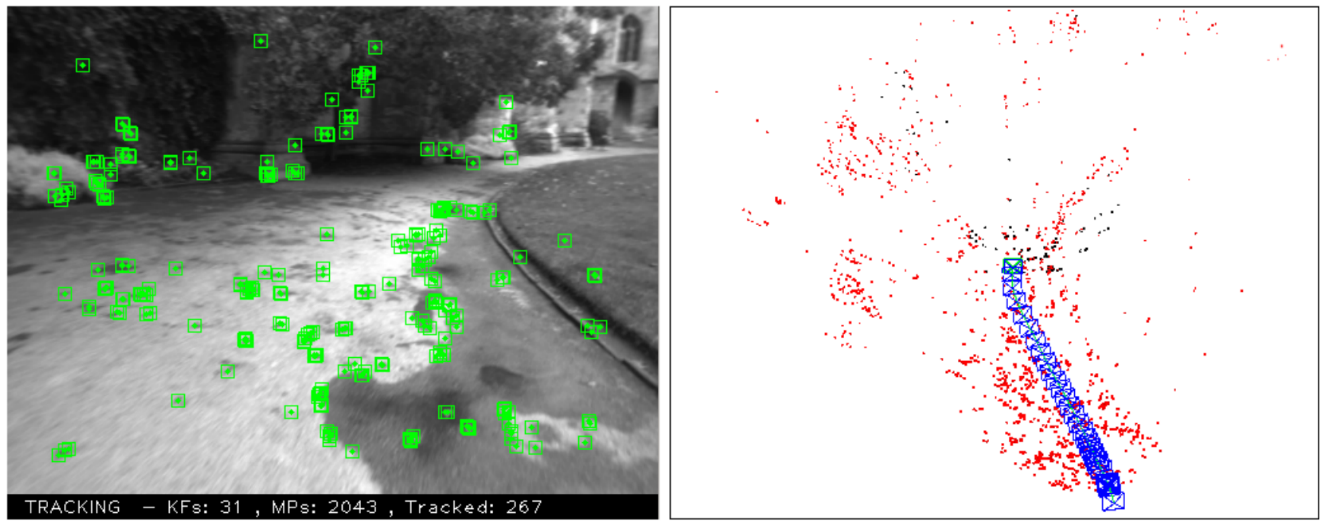
\includegraphics[scale=0.185]{./images/initialization_step}
\caption{Automatic map initialization step of ORB-SLAM, uses fundamental matrix since it has detected enough parallax. \cite{ORBSLAM}}
\label{initialization_step}
\end{figure}


\subsubsection{Initial Pose Estimation}
If tracking is successful, a constant velocity motion model is used to predict the camera pose and a guided search of the map points observed in the last frame. If tracking is lost, fame must be converted into bag of words and query the recognition database for keyframe candidates for global relocalization.

\subsubsection{Track Local Map}
Once the estimated camera pose and an initial set of feature match available, it is possible to project the map into the frame to search more map correspondences. The camera pose is finally optimized with the all map points found in the frame.

\subsubsection{New Keyframe Decision}
The last step of Tracking is to decide if the current frame is selected as a new keyframe. As mentioned in section \ref{section_introduction}, the criterion of new keyframe selection is one of six main contributions of ORB-SLAM. To insert a new keyframe, the following conditions must be met.
\begin{itemize}
\item Current frame at least 50 points
\item Current frame tracks less than $90\%$ points than reference frame.
\item More than 20 frames have passed since last global relocalization
\item More than 20 frames have passed since last key frame insertion
\end{itemize}


\subsection{Local Mapping}
Local Mapping thread performs with every new keyframe $K_i$ from tracking thread.

\subsubsection{Keyframe insertion}
Once a new frame is decided as a keyframe, it should be added into the covisibility graph. 

%
\begin{figure}[!htbp]%
\centering
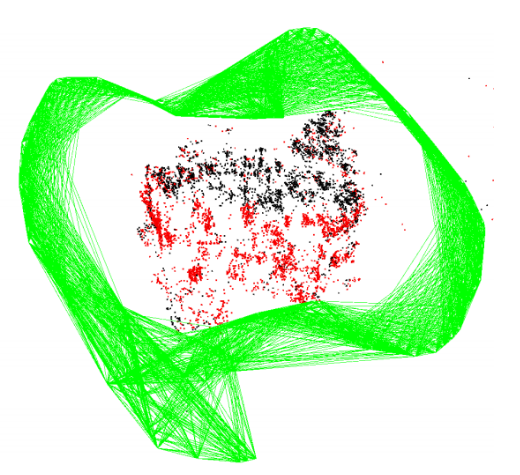
\includegraphics[scale=0.25]{./images/covisibility_graph}
\caption{A covisibility graph of ORB-SLAM after loop closing. \cite{ORBSLAM}}
\label{covisibility_graph}
\end{figure}
%
Figure \ref{covisibility_graph} shows a covisibility graph of ORB-SLAM in NewCollege dataset. After that, the bags of words' representation of the keyframe is computed, which will help triangulate new points in the data association.

\subsubsection{Recent Map Points Culling}
\label{Mappoint_culling}
To ensure the reconstructed map points are trackable and not wrongly triangulated, they must fulfill these restrictive conditions.
%
\begin{itemize}
\item The tracking must find the point in more than $25\%$ of the frames in which it is predicted to be visible.
\item If more than one keyframe  have passed from map point creation, it must be observed from at least three keyframes.
\end{itemize}
%
\subsubsection{New Map Points Creation}
New map points are created by triangulating ORB from connected keyframes in the covisibility graph. It is worth mentioning that the positive depth in both cameras, parallax, reprojection error, and scale consistency is checked to accept the new points.

%
\begin{figure}[!htbp]%
\centering
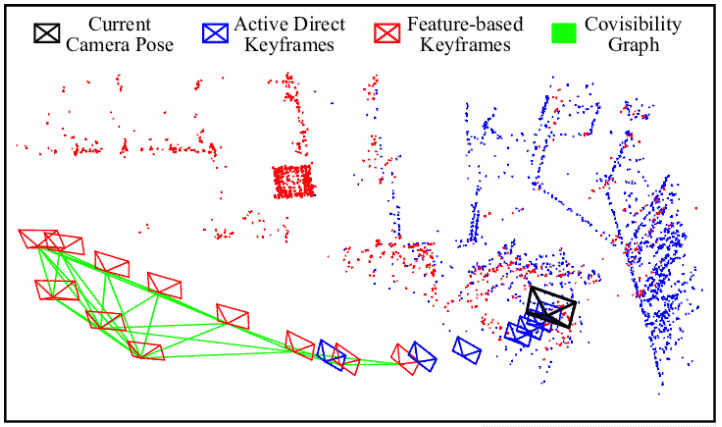
\includegraphics[scale=0.3]{./images/local_mapping}
\caption{Local mapping step creates new map points and processes local BA in the current keyframe and connected keyframes in the covisibility graph. \cite{ORBSLAM}}
\label{Local mapping}
\end{figure}
%

\subsubsection{Local Bundle Adjustment}
The local BA processes the current keyframe, all the keyframes connected to it in the covisibility graph, and all map points observed in these keyframes. Figure \ref{Local mapping} shows intuitively how the ORB-SLAM processes local mapping based on a new added keyframe.

\subsubsection{Local Keyframe Culling}
To maintain a compact reconstruction, the local mapping tries to detect redundant keyframes and delete them \cite{24}. A keyframe is discarded, when $90\%$ of map points have been seen in at least other three keyframes in the same or
finer scale.

Keyframe culling is an advantage over PTAM. As shown in figure \ref{KF_culling}, PTAM is always inserting keyframes, while ORB-SLAM is able to prune redundant keyframes and maintain a map with proper size. 
%
\begin{figure}[!htbp]%
\centering
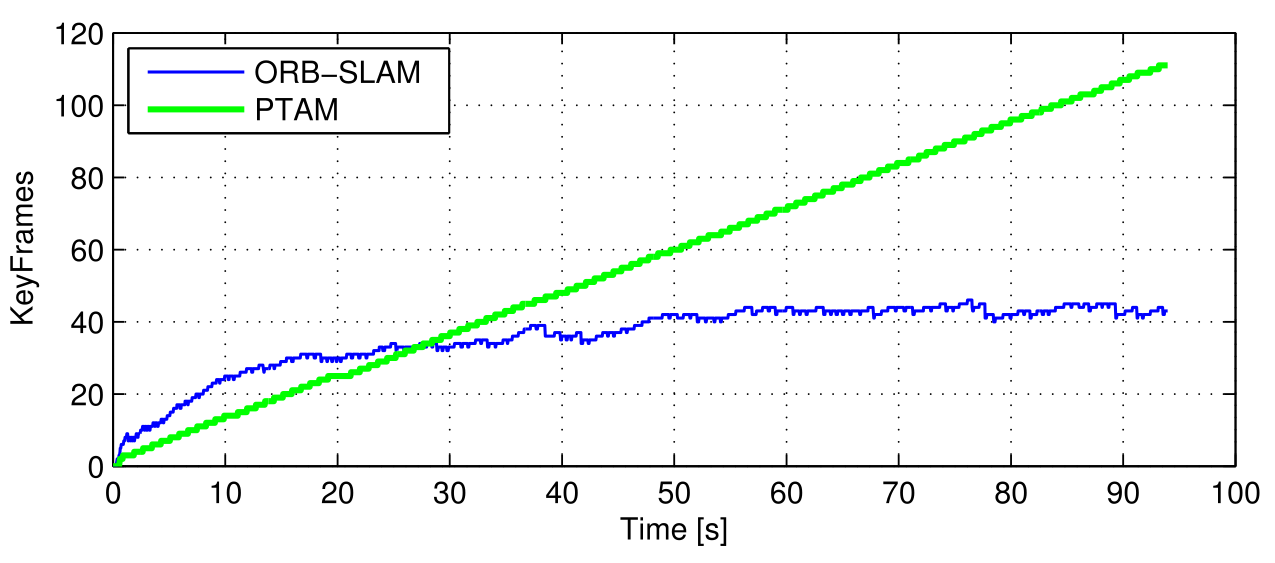
\includegraphics[scale=0.18]{./images/PTAM_ORB_KF_CULLING}
\caption{Comparsion of PTAM and ORB-SLAM in a static environment where the camera is always looking at the same place from different viewpoints. \cite{ORBSLAM}}
\label{KF_culling}
\end{figure}
%

\subsection{Loop Closing}
The loop closing thread processes the last keyframe from local mapping threads and tries to detect and close loops.
\subsubsection{Loop Candidates Detection}
A similarity score is computed between the bag of words vector of current keyframe and all its neighbbors in the covisibility graph. The lowest similarity score $s_{min}$ is retained. According to the similarity score it is possible to find several loop candidates.
%
\begin{figure}[!htbp]%
\centering
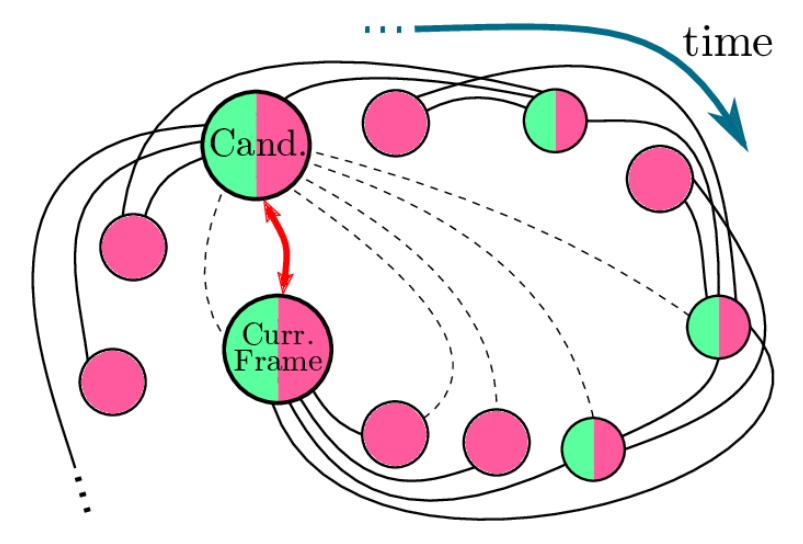
\includegraphics[scale=0.19]{./images/loop_detection}
\caption{The mechanism of loop candidates detection, similarity scores is computed between current frame and its neighbors in the covisibility graph. Loop candidates is the frame with lowest similarity score.}
\label{loop_detection}
\end{figure}
%

\subsubsection{Compute the Similarity Transformation}
In monocular SLAM, there are seven DoFs in which the map can drift: three translations, three rotations, and a scale factor \cite{6}. To compute the accumulated drift in the loop, it is needed to transform the current keyframe into the loop keyframe with a similarity transformation \cite{42}. This step also serves as a geometrical validation of the loop.

\subsubsection{Loop Fusion}
After the current frame is transformed and the accumulated drift is computed, the loop fusion step fuses duplicated map points and insert new edges in the covisibility graph. All keyframes involved in the fusion will update their edges in the covisibility graph, effectively creating edges that attach the loop closure.

\subsubsection{Essential Graph Optimization}
To process the loop closing more efficiently, an essential graph optimization is used in the loop correction step. The experiment result of ORB-SLAM shows that the essential pose optimization is so accurate that an additional full BA optimization barely improves the solution. After the optimization, each map point is transformed according to the correction of one of the keyframes that observe it \cite{6}. Figure \ref{pose_optimization} shows an intuitive example of how to process the pose graph optimization on a small loop.

%
\begin{figure}[!htbp]%
\centering
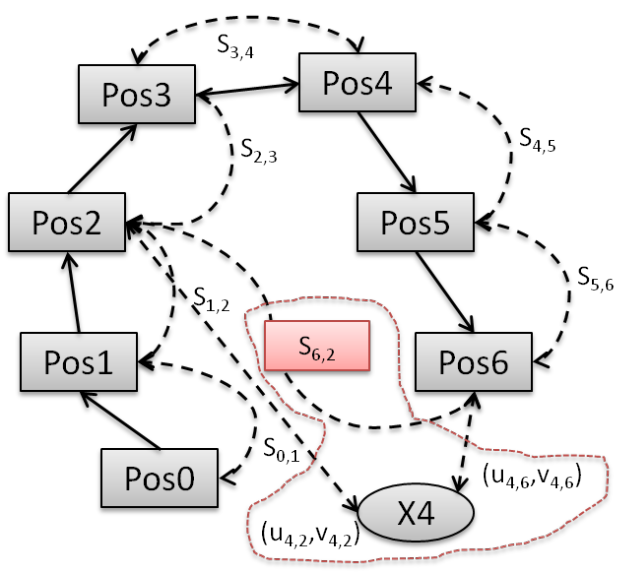
\includegraphics[scale=0.23]{./images/pose_optimization}
\caption{An example of pose optimization on an essential graph, shows pose 2 and pose 6 are potential loop closure. Pose graph optimization optimizes the pose of keyframes using reprojection error.}
\label{pose_optimization}
\end{figure}
%

\section{Performance}
\label{Performance}

The ORB-SLAM system is tested in several well-known datasets. The validation  is performed in the dataset of NewColledge \cite{39}, the general performace is evaluated according to TUM RGB-D benchmark \cite{38}, and the localization accuracy is evaluated in the sequence from the KITTI-dataset \cite{40}.

\subsection{Performance in the NewColledge Dataset \cite{39}}
The NewColledge Dataset contains a 2.2km sequence while robot traversing a campus and adjacent parks. It contains several loops and fast rotation that makes the sequence quite challenging for monocular vision. Therefore, the NewCollege dataset is an appropriate dataset to test the validation for monocular SLAM system. 

Figure \ref{new_college} shows the reconstruction and mapping before and after the loop closure. As shown in the figure, the ORB-SLAM can close the loop perfectly, which is not accomplished by other monocular SLAM systems in the NewCollege sequence yet.

%
\begin{figure}[!htbp]%
\centering
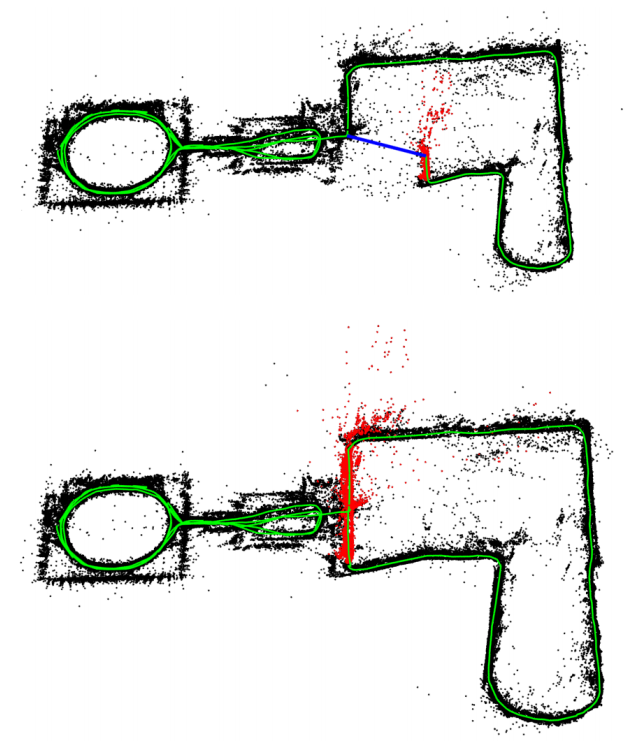
\includegraphics[scale=0.37]{./images/NewCollege}
\caption{Map before and after loop closing in the NewCollege dataset. The trajectory is drawn in green and the loop closing match is drawn in blue. \cite{ORBSLAM}}
\label{new_college}
\end{figure}
%
Besides, ORB-SLAM has excellent efficiency in tracking and mapping threads. Table \ref{Efficiency_Newcollege} shows the time cost of tracking and mapping of ORB-SLAM in the NewCollege dataset. It takes only 31.6 ms for the tracking thread, which meets the requirement of real-time operation. Local BA takes over 300 ms. However, it is a nonlinear optimization process, which does not need to run simultaneously. Therefore, ORB-SLAM is a well-performed real-time localization method.
%
\begin{table}[h!]
\caption{Tracking and Mapping Time in NewCollege.}
\label{Efficiency_Newcollege}
\centering
\begin{tabular}{ l l c } 
\hline
 \hline
 Thread & Operation & Mean (ms) \\ 
 \hline
 Tracking & ORB Extraction & 11.42\\ 
 		  & Initial Pose Estimation & 3.45\\ 
 		  & Track Local Map & 16.01\\ 
 		  & Total & 31.60\\ 
 Local Mapping & Keyframe Insertion & 11.88\\ 
 		       & Map Point Culling & 3.18\\ 
 		       & Map Point Creation & 72.96\\ 
 		       & Local BA & 360.41\\
 		       & Keyframe Culling & 15.79\\
 		       & Total & 464.27\\
\hline
 \hline
\end{tabular}
\end{table}
%
 
\subsection{Performance in the TUM RGB-d Dataset \cite{38}}
The TUM RGB-D benchmark is a unique dataset to evaluate the accuracy of vision localization because it provides several sequences with accurate ground truth obtained with an external motion capture system. Besides, it is possible to compare the result with other SLAM systems such as LSD-SLAM and PTAM in the TUM RGB-D dataset, which lets the performance more intuitively presented.

Table \ref{TUM Dataset} shows a comparison of localization error in centimeter of ORB-SLAM \cite{ORBSLAM}, LSD-SLAM \cite{LSD}, and PTAM \cite{PTAM}. Intuitively, the ORB-SLAM has less localization error at most places in the TUM RGB-D sequence. Generally, ORB-SLAM has the best localization performance among other SLAM systems.

\begin{table}[h!]
\caption{Localization Error of ORB-SLAM, LSD-SLAM, and PTAM in the  TUM RGB-D Benchmark.}
\label{TUM Dataset}
\centering
\begin{tabular}{ l c c c } 
\hline
 \hline
 Position & ORB-SLAM & PTAM & LSD-SLAM\\ 
 \hline
 Position 1	& \textbf{0.90} & 1.15 & 9.00\\ 
 Position 2	& 0.30 & \textbf{0.20} & 2.15\\ 
 Position 3	& \textbf{2.99} & X & 38.07\\ 
 Position 4 & \textbf{1.69} & X & 10.65\\ 
 Position 5	& 3.81 & \textbf{2.63} & X\\ 
 Position 6 & \textbf{0.88} & X & 4.57\\ 
 Position 7 & \textbf{3.45} & X & 38.53\\
 Position 8 & \textbf{1.39} & 2.74 & 7.54\\
 Position 9 & \textbf{0.77} & 0.93 & 7.95\\
\hline
 \hline
\end{tabular}
\end{table}
%

\subsection{Performance in the KITTI Dataset \cite{40}}
The KITTI dataset is an appropriate large-scale dataset to test the performance of SLAM systems. It is a extremely challenging dataset for monocular vision slam due to fast rotations and relatively high car speed. The results show that ORB-SLAM is a accurate and efficient SLAM system.


\section{Implementation} 
In this section, the lesson lerned about the function and the structure implemented in the ORB-SLAM is introduced. It is generous of the author that he published all code open-sourced \cite{ORB2}. Since ORB-SLAM is such a well-performed SLAM system, it is an excellent chance to analyze the code and reproduce the SLAM system. 

\subsection{Main Procedure}
Essential functions are introduced in this section. ORB-SLAM supports now monocular, stereo, and RGB-D camera system. In the following sections, the only implementation in the monocular system is discussed.

\subsubsection{System.cpp}

At first use function \textit{GrabImageMonocular()} to insert images. Images are converted in gray-scale and named \textit{mImGray}. Besides, an ORB vocabulary is loaded in this step. Keyframes and map are created and all three threads introduced in section \ref{section3} are initialized.

\subsubsection{Tracking.cpp}
Firstly, use \textit{MonocularInitializer()} to initialize the tracker. The frame with features extracted less than 100 is dropped. Besides, the tracker needs 2 frames to perform the initialization step.

Create object \textit{mpIniORBextractor()} from class \textit{ORBextractor} as a feature extractor. The class is implemented separately in script \textit{ORBextractor.cpp}.

Use heuristirc introduced in section \ref{map_init} to choose the Homography or Fundamental matrix to compute relative motion between two frames and map points. This procedure is implemented in \textit{mpInitializer()}. Use \textit{CreateInitialMapMonocular()} to store the reconstructed 3D points into keyframes and the map.

\subsubsection{LocalMapping.cpp}
Use \textit{InsertKeyFrame()} and \textit{CheckNewKeyFrames()} to insert new keyframes from the tracking thread and check if all new keyframes are added. After that, links between keyframes are updated in the covisibility graph and essential graph.

Use of \textit{MapPointCulling()} can elinimate the map points added in the last step with low quality. The criterion of good map points are introduced in section \ref{Mappoint_culling}. Each corresponding points in keyframes must be triangulated to create more map points. 

The last step in the local mapping thread is implemented in \textit{KeyFrameCulling()}. If $90\%$ of map points in a keyframe can be detected by at least other three keyframes, this keyframe is redundant and must be culled.

\subsubsection{LoopClosing.cpp}
Similar to the local mapping thread, the loop closing thread is based on each new keyframe. Therefore it uses same functions \textit{InsertKeyFrame()} and \textit{CheckNewKeyFrame()} to insert and check new keyframes.

In function \textit{DetectLoop()}, the reference BoW similarity score is computed between the new keyframe and all keyframes in the covisibility graph. After that, the keyframe with lowest similarity score is chosen and added into loop candidates \textit{vpCandidateKFs}. However, if there is no loop candidate, this function only adds the new keyframe and return false.

For each loop candidate the consistency with previous loop candidates is checked. Each loop candidate and connected keyframes build cobisibility group \textit{spCandidateGroup}. The consistent loop must be detected in several consecutive keyframes to be accepted.

Use \textit{ComputeSim3()} based on RANSAC to compute the sim3 between current keyframe and loop candidate. Based on the estimated sim3, it is possible to project 3D points and compute more accurate sim3 using optimization method. The solver of sim3 is implemented separately in script \textit{Sim3Solver.cpp}. 

\textit{CorrectLoop()} is the function which is implemented to fuse the loop candidates and duplicated map points. Based on the solved sim3 and relative pose, the pose of keyframe and detected map points is adjusted. The map points of loop candidate and current keyframe are machted and the covisibility graph is updated. After the pose optimization based on the essential graph, a global bundle adjustment is performed.

\subsubsection{Others}

Except the main procedure and threads, there are still many implemented function of ORB-SLAM. They are all published on GitHub site of author.

\subsection{Robot Operating System}
ORB-SLAM is implemented in ROS (Robot Operating System). ROS is an operating system in concept because it provides all the services such as hardware abstraction, low-level device control, implementation of commonly-used functionality, message-passing between processes, and package management.


\subsection{Demo}
There is a ROS implementation of the ORB-SLAM real-time SLAM library for Monocular, Stereo and RGB-D cameras available, that computes the camera trajectory and a sparse 3D reconstruction. It is able to detect loops and relocalize the camera in real time. This demo is extremly user-friendly because all data I/O is handled via ROS topics. For vizualization people can use RViz. 

After the installation of ROS and other required packages, user can launch ORB-SLAM by given
%
\begin{lstlisting}
rosrun ORB_SLAM2 Mono PATH_TO_VOCABULARY 
PATH_TO_SETTINGS_FILE
\end{lstlisting}
%
in terminal. The input images can be inserted either from a ROS bag such as TUM RGB-D dataset, or a commonly used mono camera. As shown in figure \ref{example}, the ORB-SLAM is launched successfully. It is connected with a webcam and has a robust tracking performance. If the camera moves too fast, the ORB-SLAM could lose tracking. However, it can still relocalize the camera position in a tiny time, which is an advantage of ORB-SLAM introduced in section \ref{section_introduction}.


\begin{figure}[!htbp]
\centering
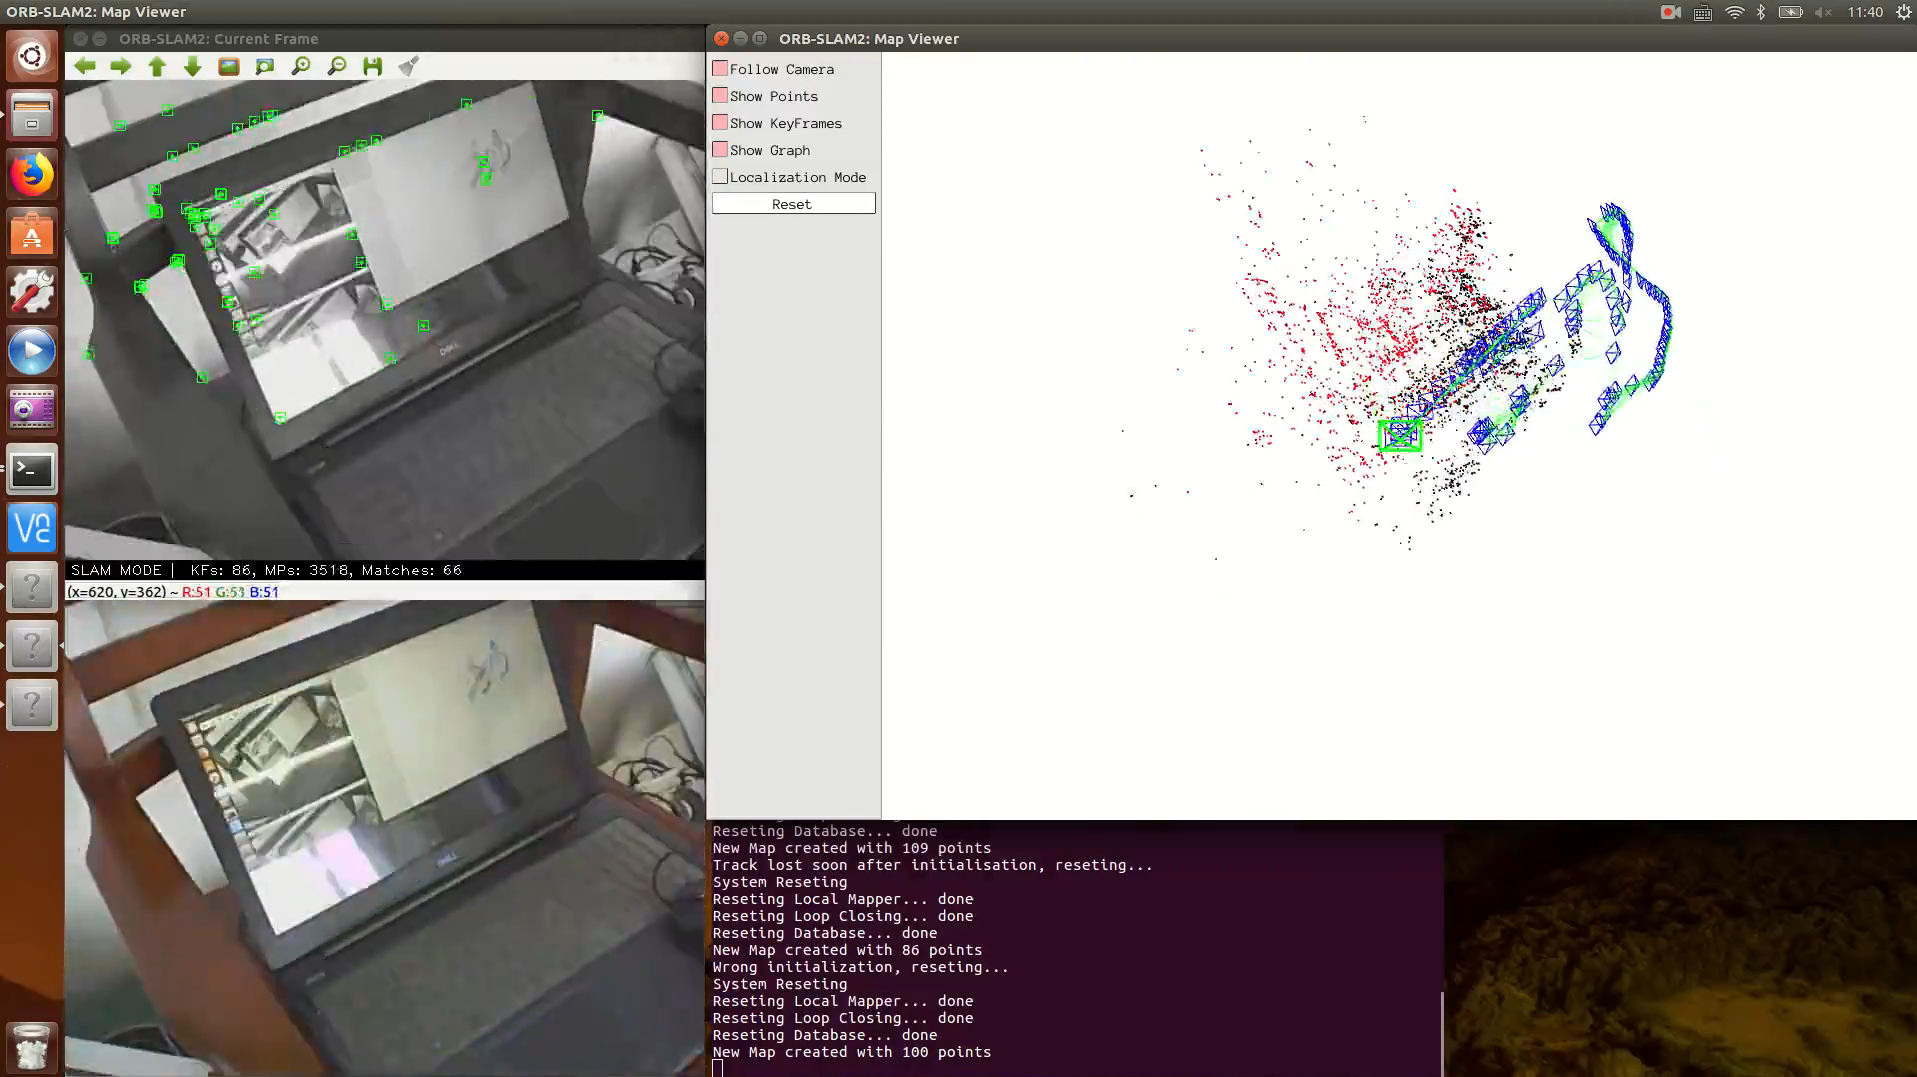
\includegraphics[scale=0.128]{./images/ORB_example}
\caption{ORB-SLAM using mono camera, launched in ROS environment.}
\label{example}
\end{figure}

\section{Overview and Outlook}

In this section, also the last chapter of the paper, a short summary of seminar sensors in robots and some continuing concepts and work regarding the visual SLAM methods are given.

\subsection{Summary}
The comparison of ORB-SLAM and other SLAM systems is given in section \ref{Performance}. It is obvious that the ORB-SLAM is the state-of-the-art SLAM method at that time. Besides, it has a very user-friendly implementation, which allows people to launch and improve the system quickly. 

\subsection{Future Work}
There are still several aspects, which ORB-SLAM should improve.
\subsubsection{Accuracy}
The ORB extractor is extremely efficient. However, the accuracy of ORB-SLAM can be improved incorporating points at infinity in the tracking.
\subsubsection{Reconstruction}
The reconstructed map is sparse. As known to all, a dense map is usually more intuitive and useful. Luckily, the sparse map of ORB-SLAM can be an excellent initial guess and skeleton, on top of which a dense and accurate map of the scene can be built.
\subsubsection{Semantic SLAM}
The SLAM system can be nowadays combined with deep learning. Using semantic segmentation in SLAM brings advantages from two aspects.
%
\begin{itemize}
\item Semantic supports SLAM: Give every object detected a label helps in loop detection and bundle adjustment optimization.
\item SLAM supports Semantic: Compute the position of objects helps humans save time on labeling in the training dataset.
\end{itemize}
%
\begin{figure}[!htbp]
\centering
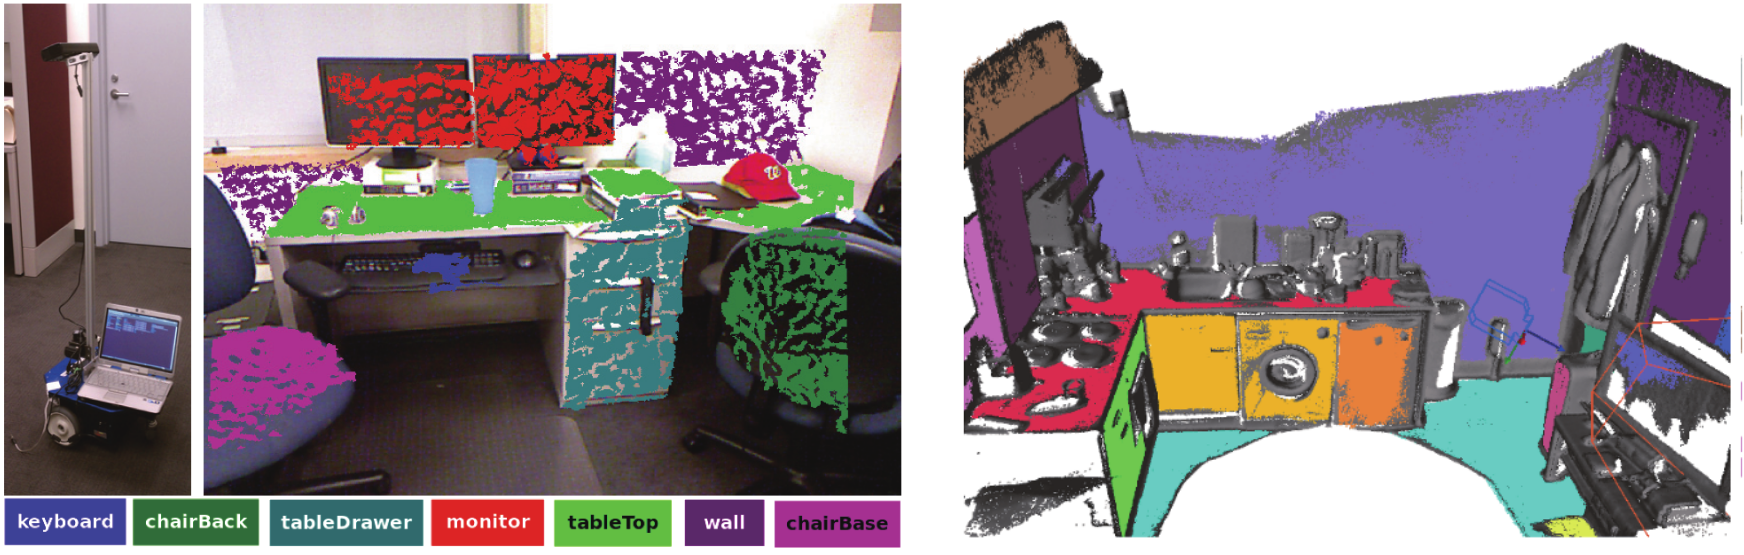
\includegraphics[scale=0.14]{./images/semantic_slam}
\caption{An example of Semantic SLAM. \cite{Semantic}}
\label{semantic_slam}
\end{figure}


\section*{ACKNOWLEDGMENT}
Personally, it is my first seminar paper. To be honest, this is the first paper I read about SLAM, and I am very interested in this topic. It is worth investing the time of a month to read the paper and prepare for the presentation. 

Due to the pandemic of the coronavirus, it is not possible to hold the seminar as usual. Therefore, I want to give a special thanks to our supervisor Peter Gawronski, who always answers questions in the shortest time and ensures us having a successful online presentation. I appreciate our professor Burschka, who attended the seminar every time and gave us some guidance in research.

%%%%%%%%%%%%%%%%%%%%%%%%%%%%%%%%%%%%%%%%%%%%%%%%%%%%%%%%%%%%%%%%%%%%%%%%%%%%%%%%
\printbibliography




\end{document}
